% this file is called up by thesis.tex
% content in this file will be fed into the main document

%: ----------------------- name of chapter  -------------------------
\chapter{Implementacja projektów} % top level followed by section, subsection


%: ----------------------- paths to graphics ------------------------

% change according to folder and file names
\ifpdf
    \graphicspath{{5/figures/PNG/}{5/figures/PDF/}{5/figures/}}
\else
    \graphicspath{{5/figures/EPS/}{5/figures/}}
\fi

%: ----------------------- contents from here ------------------------


W rozdziale trzecim zostały przedstawione wymagania funkcjonalne i niefunkcjonalne stawiane przed przykładowymi aplikacjami mogącymi korzystać z systemu którego implementacja była celem tej pracy. Niniejszy rozdział opisuje sposób implementacji tych aplikacji.
\section{Automatyczne dyktando}
Automatyczne dyktando, jak już zostało opisane w rozdziale trzecim, jest to prosty serwis internetowy umożliwiający użytkownikowi ćwiczenie ortografii. Jak większość współczesnych aplikacji internetowych ma budowę warstwową, składa się z 3 warstw:
\begin{itemize}
	\item prezentacji,
	\item logiki biznesowej,
	\item komunikacji z serwisem UniversalSynthesizer.
\end{itemize}
\begin{figure}[!h]
	\centering
	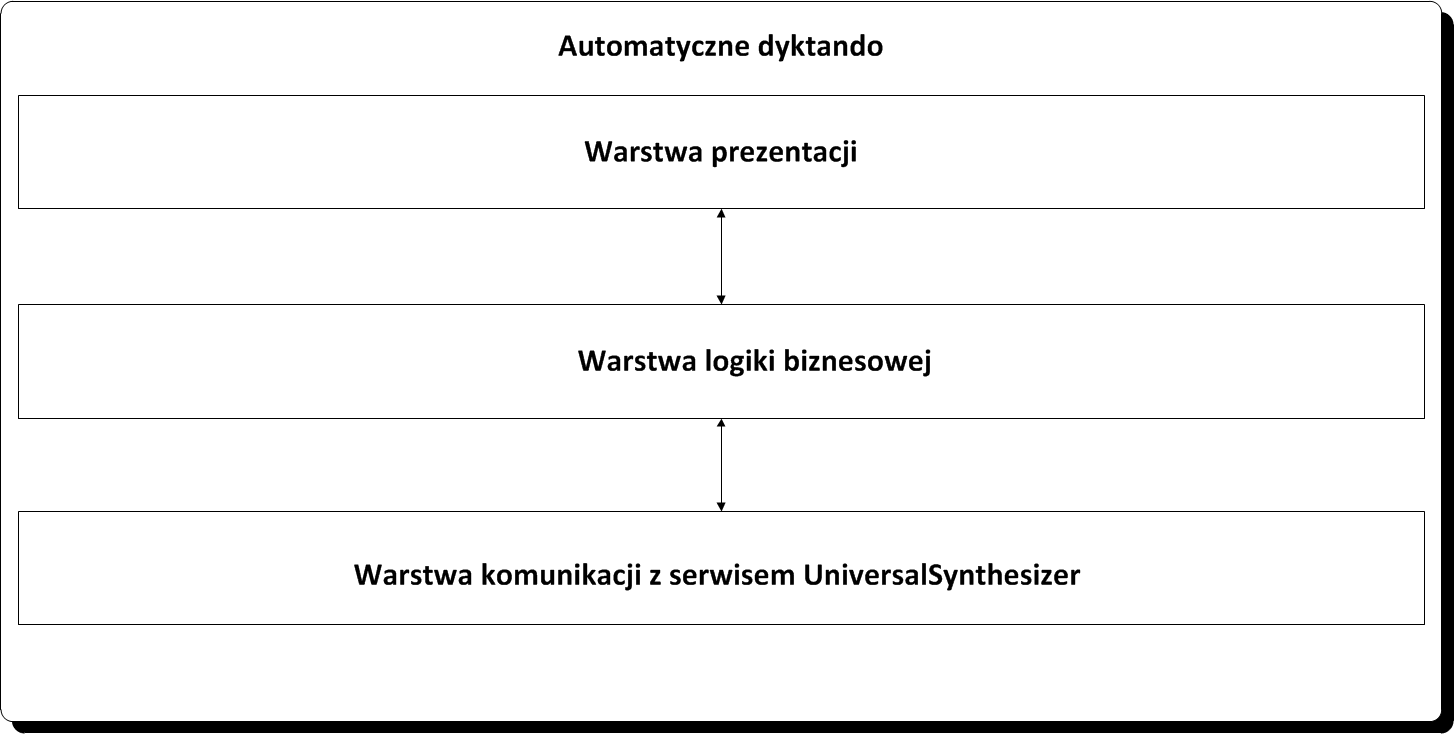
\includegraphics[scale=0.45]{automatyczneDyktandoArchitektura.png} 
	\caption{Automatyczne Dyktanto Architektura}
\end{figure}
Do stworzenia szkieletu tej aplikacji wykorzystano framework Spring MVC, do tworzenia widoków framework Freemarker a do komunikacji z serwisem UniversalSynthesizer bibliotekę jersey-client będącą implementacją JAX-RS. 
\newpage
\subsection{Warstwa prezentacji}
W skład warstwy prezentacji wchodzą trzy pliki *.ftl reprezentujące 3 strony:
\begin{itemize}
	\item strona główna - umożliwiająca podanie tekstu lub też załadowanie pliku tekstowego, który posłuży jako treść dyktanda
	\item strona z odtwarzaczem - umożliwiająca odsłuchanie tekstu i napisanie jego transkrypcji
	\item strona z wynikami - pokazująca ilość błedów popełnionych przez użytkownika
\end{itemize}
\begin{figure}[!h]
	\centering
	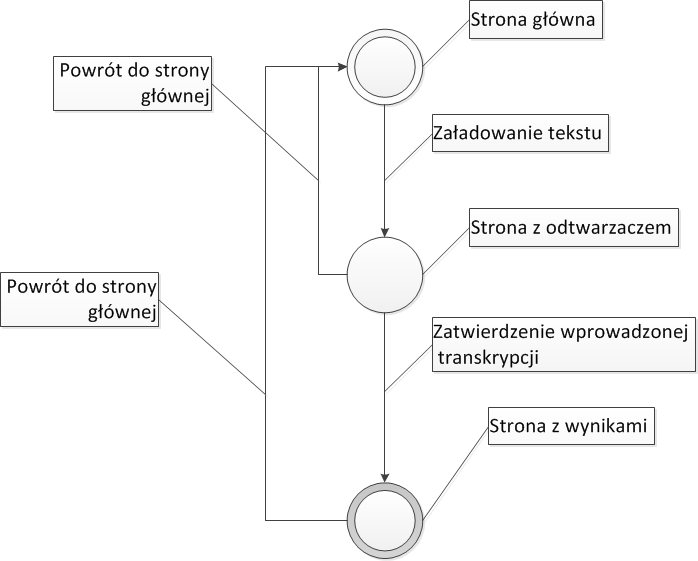
\includegraphics[scale=0.45]{AutomaticDictandoControlDiagram.png} 
	\caption{Automatyczne Dyktanto - diagram przepływu sterowania}
\end{figure}
\newpage
Do każdej ze stron jest przypisany jeden kontroler napisany przy użyciu Spring MVC, dodatkowo istnieje także kontroler odpowiedzialny za ładowanie plików na serwer co w sumie daje nam 4 kontrolery:
\begin{itemize}
	\item MainController - kontroler strony głównej
	\item TextUploadController - kontroler odpowiedzialny za ładowanie treści dyktanda w postaci tekstu na serwer
	\item FileUploadController - kontroler odpowiedzialny za ładowanie treści dyktanda w postaci pliku tekstowego na serwer
	\item UserTextUploadController - kontroler odpowiedzialny za ładowanie i sprawdzenie poprawności tranksrypcji stworzonej przez użytkownika
\end{itemize}
Zastosowanie wspomnianych framework'ów oraz wzorca Model-View-Controller bardzo uprościło implementację. Freemarker mimo, iż wydaje się bardzo prostym narzędziem w istocie posiada dużą moc i bardzo dobrze współpracuje ze Spring'iem. Dzięki Spring MVC i gotowym implementacją kontrolerów wbudowanych w ten framework, kod wymagany do działania aplikacji został sprowadzony do minimum. \\
Możliwość użycia adnotacji takich jak:
\begin{itemize}
	\item @Controller
	\item @RequestMapping
	\item @RequestParam
\end{itemize}
jeszcze bardziej ułatwiła implementację i zwiększyła czytelność klas użytych w tej warstwie.
\subsection{Warstwa logiki biznesowej}
Warstwa logiki biznesowej składa się z 2 klas:
\begin{itemize}
	\item TextIntoSoundTrasformer
	\item TextCorrector
\end{itemize}
Pierwsza z wyżej wymienionych zajmuje się propagacją tekstu dyktanda z warstwy widoków do warstwy komunikacyjnej w celu otrzymania adresu pliku dźwiękowego. Funckjonalność tej klasy ogranicza się do obcięcia białych znaków z początku i końca łańuchu znakowego.\\
Druga natomiast, jak sama nazwa wskazuje, zajmuje się sprawdzaniem poprawności transkrypcji stworzenej przez użytkownika poprzez porównanie jej z oryginalnym tekstem i znalezienie różnic. W tym celu stosuje jedną z najpopularniejszych i najskuteczniejszych metryk a mianowicie: Dystans Levenshtein'a. W skrócie, dystans ten można zdefiniować jako najmniejszą możliwą liczbę zmian jaka jest potrzebna by jeden z łańcuchów znaków zmienić w drugi. Operacje które wolno stosować to:
\begin{itemize}
	\item wstawienie znaku
	\item usunięcie znaku
	\item zamiana znaku
\end{itemize}
Jest to algorytm dynamiczny o złożoności \textbf{O(M*N*max(M,N))} gdzie M i N to długości łańuchów znaków. Algorytm ten można ulepszyć stosując koncepcje Lowrance'a i Wagner'a. W najgorszym wypadku złożoność ulepszonego algorytmu wynosi \textbf{O(M*N)}.
\subsection{Warstwa komunikacji z serwisem UniversalSynthesizer}
Warstwa komunikacji składa się z jednej klasy:
\begin{itemize}
	\item UniversalSynthesizerConnector
\end{itemize}
Zadaniem obiektu tej klasy (dzięki użyciu Spring IOC mamy tylko jeden obiekt tej klasy, a więc korzystamy z wzorca Singleton) jest uzyskanie połączenia z serwisem UniversalSynthesizer, wysłanie zapytania typu POST  z parametrem "text" którego wartością jest tekst który użytkownik załadował na serwer (niezależnie od tego, którego sposobu ładowania tekstu użył użytkownik) oraz odebranie odpowiedzi będącej adresem URL do pliku dźwiękowego.\\
Klasa ta do komunikacji z serwisem wykorzystuje bibliotekę jersey-client. Jest to gotowa, otwarta implementacja JAX-RS. Pozwala ona w prosty, bezpieczny, szybki i skuteczny sposób łączyć się z serwisami działającymi zgodnie z architekturą REST.    
\section{LektorsRSS}
Krótki opis o raz wymagania stawiane przed tą aplikacją zostąły podane w rodziale trzecim. Aplikacja ta podobnie jak Automatyczne Dyktando ma budowę warstwową. W jej skład wchodzą cztery warstwy:
\begin{itemize}
	\item prezentacji,
	\item logiki biznesowej,
	\item danych.
\end{itemize}
\begin{figure}[!h]
	\centering
	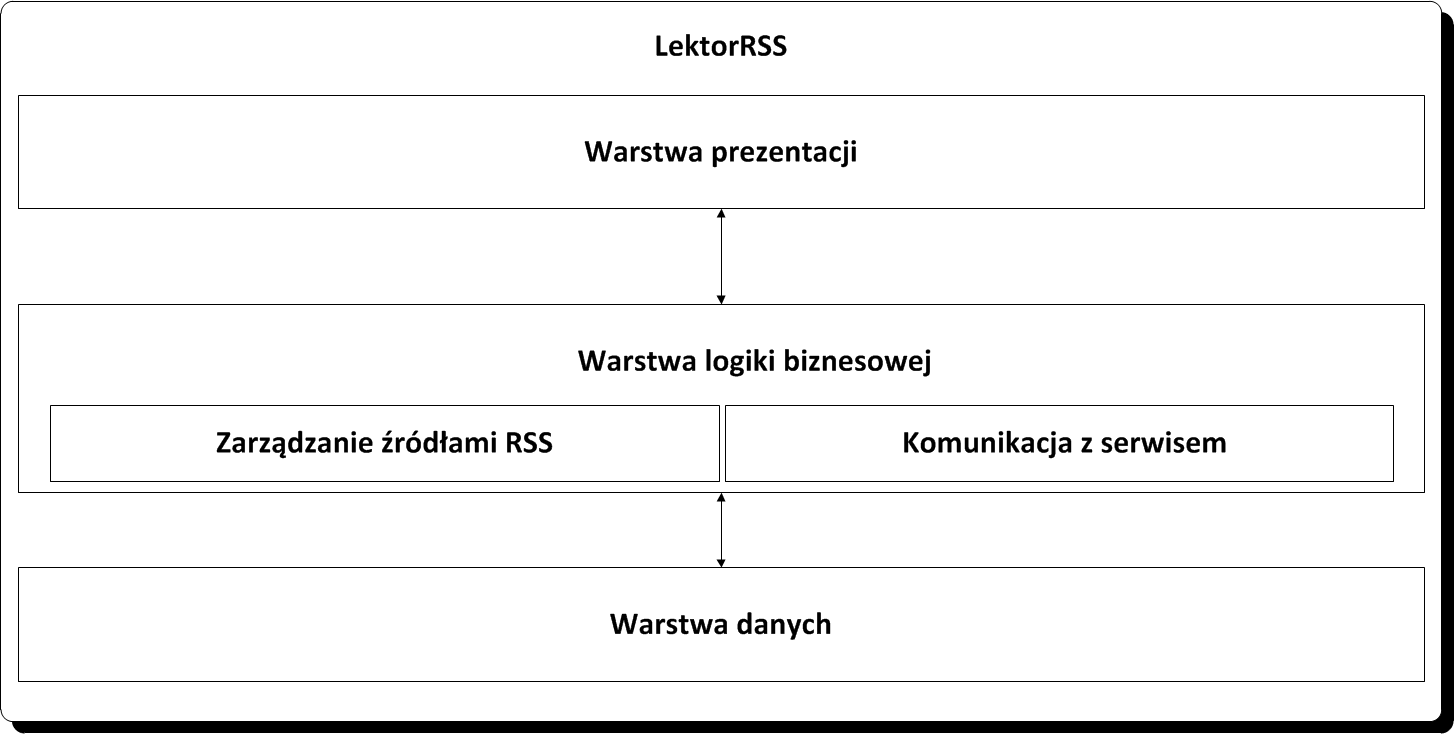
\includegraphics[scale=0.45]{LektorRSSArchitecture.png} 
	\caption{LektorRSS Architektura}
\end{figure}
\newpage
Podobnie jak w przypadku Automatycznego Dyktanda do stworzenia szkieletu aplikacji wykorzystano framework Spring MVC, do stworzenia widoków framework Freemarker,  do komunikacji z serwisem UniversalSynthesizer bilbiotekę jersey-client. W przypadku tej aplikacji istnieje konieczność korzystania z bady danych, wybór padł na MongoDB oraz Google Morphia jako bibliotekę do komunikacji między aplikacją a bazą danych. Do komunikacji z RSS wykorzystano bibliotekę ROME.
\subsection{Warstwa prezentacji}
Interfejs aplikacji ogranicza się do jednej strony głównej, która umożliwia modyfikowanie listy interesujących nas źródeł RSS, odsłuchanie nowej wiadomości o ile taka się pojawiła oraz zmianę częstotliwości sprawdzania źródeł w poszukiwaniu nowości.
Do wygenerowania tej stworzomy został tylko jeden plik *.ftl , który obsługiwany jest jednak aż przez 3 kontrolery:
 \begin{itemize}
	\item MainController - odpowiedzialny za wyrenderowanie listy źródeł interesujących dla użytkownika
	\item ManageFeedsSourcesController - odpowiedzialny za zarządzanie źródłami, czyli dodawanie i usuwanie oraz za ustawianie interwału
	\item UpdateFeedController - kontroler którego głównym i jedynym zadaniem jest odpytywanie źródeł w celu sprawdzenia czy nie pojawiła się nowa wiadomość
\end{itemize}
Jak łatwo się domyślić, istotnym elementem warstwy prezentacji jest wykorzystanie technologii AJAX. Jest ona wykorzystana do dynamicznego modyfikowania listy źródeł RSS, automatycznego odpytywania serwera o nowe wiadomości oraz, w przypadku pojawienia się nowej, do wygenerowania odtwarzacza który ją odczyta.
\begin{figure}[!h]
	\centering
	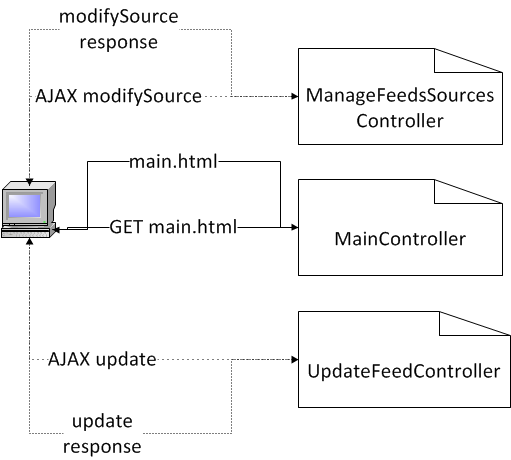
\includegraphics[scale=0.65]{LektorRSSKomunikacja.png} 
	\caption{LektorRSS diagram komunikacji}
\end{figure}
\subsection{Warstwa logiki biznesowej}
Warstwa logiki biznesowej składa się z dwóch klas:
\begin{itemize}
	\item FeedsUpdaterImplementation
	\item UniversalSynthesizerConnector
\end{itemize}
FeedsUpdaterImplementation jak nazwa wskazuje zajmuje się odpytywaniem źródeł RSS w poszukiwaniu nowych wiadomości. 
Do pobierania oraz parsowania wiadomości używa otwartej, prostej w obsłudze oraz dość wydajnej biblioteki ROME. Klasa ta wykorzystuje bazę danych do zapamiętywania ostatniej wiadomości z konkretnego źródła. Jeżeli przy sprawdzaniu okaże się, że wiadomość jest różna od przechowywanej w bazie, to jest ona przekazywana do klasy odpowiedzialnej za komunikację z serwisem UniversalSynthesizer i, w dalszej kolelności, w formie dźwiękowej przekazana do użytkownika, a także zastępuje starą wiadomość powiązaną z konkretnym źródłem w bazie danych.
Klasa UniversalSynthesizerConnector służy do komunikacji z serwisem, celem zamiany tekstu wiadomości na dźwięk. Implementacja jest bardzo podobna do bliźniaczej klasy opisanej przy okazji projektu "Automatyczne Dyktando", podobnie jak w tamtym projekcie, wykorzystuje ona bibliotekę jersey-client. Ponieważ obie korzystają z tego samego zewnętrznego serwisu to budowa zapytania jest bardzo podobna.
\subsection{Warstwa danych}
W skład warstwy danych wchodzi model danych oraz klasy nim zarządzające czyli tak zwane DAO. W aplikacji tej model danych składa się tylko z jednej klasy:
\begin{itemize}
	\item FeedSource
\end{itemize}
Oprócz standardowego pola id, posiada ona dwa atrybuty więcej:
\begin{itemize}
	\item source - pole typu String, reprezentuje adres źródła RSS
	\item lastFeed - pole typu String, służy do przechowywania treści ostatniej wiadomości pobranej z tego źródła
\end{itemize}
\begin{figure}[!h]
	\centering
	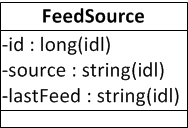
\includegraphics[scale=0.65]{FeedSourceDiagram.png} 
	\caption{LektorRSS model danych}
\end{figure}
\newpage
Dzięki zastosowaniu biblioteki Morphia, implementacja DAO bardzo się uprościła. Aby korzystać z operacji typu CRUD wystarczającym okazało się stworzenie nowych klas dziedziczących po odpowiednich klasach oraz ustawienie im odpowiednich typów. 
\begin{figure}[!h]
	\centering
	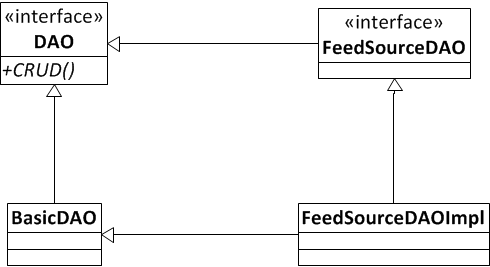
\includegraphics[scale=0.65]{LektorRSSDiagramKlasDAO.png} 
	\caption{LektorRSS diagram klas należących do DAO}
\end{figure}

\section{LektorSMS}




% ---------------------------------------------------------------------------
%: ----------------------- end of thesis sub-document ------------------------
% ---------------------------------------------------------------------------

